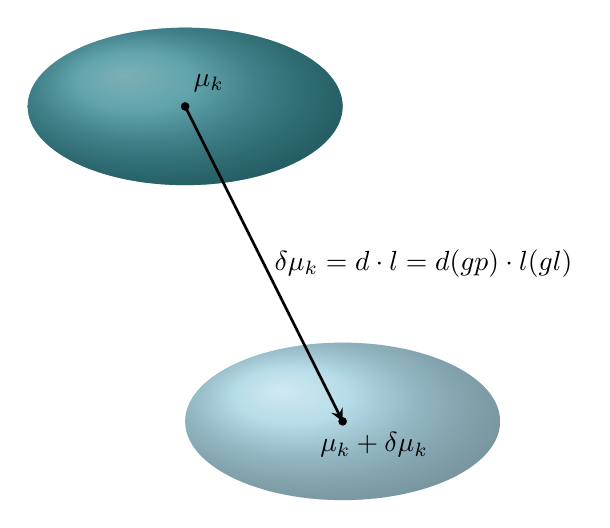
\begin{tikzpicture}
    \def\x{0}
    \def\y{2}
    \def\xf{2}
    \def\yf{-2}
    \def\sx{2}
    \def\sy{1}
    % Draw the larger ellipse labeled X_μ
    % \draw[thick] (\x, \y) ellipse ({\sx} and {\sy});
    \def\dx{1}
    \def\dy{1}
    % \def\s{1.5}
    \def\gop{0.5}
    \definecolor{dark_cyan}{RGB}{5, 104, 110}
    \definecolor{light_cyan}{RGB}{173, 216, 230}
    
    \fill[dark_cyan] (\x, \y) ellipse ({\sx} and {\sy});
    \shade[ball color=light_cyan, opacity=\gop] (\x, \y) ellipse ({\sx} and {\sy});
    \fill (\x, \y) circle (1.5pt); % Point at the center of X_μ
    \node at (\x + 0.3, \y + 0.3) {\textbf{$\mu_k$}};
    
    % Draw the smaller dashed ellipse labeled "interior"
    \fill[light_cyan] (\xf, \yf) ellipse ({\sx} and {\sy});
    \shade[ball color=light_cyan, opacity=\gop] (\xf, \yf) ellipse ({\sx} and {\sy});
    \fill (\xf, \yf) circle (1.5pt); % Point at the center of interior
    % \node[below] at (0, -2.5) {\textit{interior}};
    
    % Draw points and arrow
    \fill (\x, \y) circle (1.5pt); % Point at the center of X_μ
    \fill (\xf, \yf) circle (1.5pt); % Point at the center of interior
    \draw[thick, ->, >=stealth, line width=1pt] (\x, \y) -- (\xf, \yf) node[midway, right] {$\delta \mu_k = d \cdot l = d (gp) \cdot l(gl)$};
    % \draw[thick, ->, >=stealth, line width=2.5pt] ({\xf + (\x - \xf) * 0.000001}, {\yf + (\y - \yf) * 0.000001}) -- (\xf, \yf);
    
    \node at (\xf+0.4, \yf - 0.3) {\textbf{$\mu_k + \delta \mu_k$}};
    % Annotate components of the formula
    % \node[right] at (\xf, \yf + 1) {$d$ (growth direction probabilities)};
    % \node[right] at (\xf, \yf + 0.5) {$l(s)$};
\end{tikzpicture}